\chapter{Test des Systems}
\label{chapter:testing}

	\todo{Eventuell Anforderungen, die ominös angesprochen werden, direkt referenzieren.}
	Das Testen des Softwaresystem wurde in drei Aufgabenbereiche unterteilt.
	Zuerst wurde das Frontend durchgängig getestet.
	Anschließend wurde das Backend überprüft.
	Letztendlich wurde der Algorithmus und die Auswirkung diesen auf Richtigkeit untersucht.\newline
	
	Es gibt außerdem einige Verweise auf Testskripts, welche mit Laravel Dusk ausgeführt werden können.
	Um diese auf einer lokal laufenden Kopie auszuführen, kann das Skript "runTests.sh" in einem Terminal genutzt werden.\newline
	
	\section{Frontend}
		Um das Frontend ordnungsgemäß zu testen, wurden verschiedene Testobjekte betrachtet.
		Im Folgenden werden diese erläutert.
		
		\subsection{Homepage}
			Um die Homepage zu testen, reichte es aus, den Header zu überprüfen.
			Dies bedeutet, dass sowohl die Textfelder des Headers, also ''Start'', ''Kursübersicht'', ''Meine Präferenzliste'', und ''Ergebnis sehen'', als auch die Reihenfolge derer überprüft wurden.
			Zusätzlich wurden die Texte der Buttons, ''Anmelden'' und ''Registrieren'', und die Reihenfolge geprüft.
			Dies geschieht in dem Testfall \textit{HomepageTest}.\newline
		
		\subsection{Registrierung}
			Der Testfall \textit{RegisterTest} verifiziert, dass ein Nutzer sich ordnungsgemäß registrieren kann und anschließend auch mit diesen Daten anmelden kann.
			Dafür klickt der automatisierte Nutzer auf den ''Registrieren''-Button der Homepage und registriert sich.
			Anschließend ruft der User die Login-Seite auf und meldet sich an.
			Ein erfolgreicher Login wird durch die Abwesenheit des ''Anmelden''-Buttons sicher gestellt.
			Zu Ende des Testfalls wird der neu registrierte Nutzer gelöscht.\newline
		
		\subsection{Login}
			Der daran anschließende Testfall ist \textit{LoginTest}.
			Dieser testet, dass ein bereits registrierter Benutzer sich anmelden kann.
			Dafür wird zuerst ein Nutzer in der Datenbank kreiert.
			Dieser automatische User öffnet die Login-Seite und gibt die Daten des kreierten Nutzers ein.
			Der erfolgreiche Login wird durch die Abwesenheit des ''Anmelden''-Buttons sicher gestellt.
			Zu Ende des Testfalls wird der kreierte Nutzer aus der Datenbank gelöscht.\newline
		
		\subsection{Kursübersicht}
			Manuell getestet wurde die Kursübersicht.
			Um dies zu testen, wurden zuerst Kurse im Backend erstellt.
			Diese wurden anschließend im Frontend unter dem Menüpunkt ''Kursübersicht'' überprüft.
			Hierbei ist es wichtig, dass in dem Einführungstext der Übersicht das korrekte Jahr steht.
			Anschließend wurde die Vorschau für die Kurse kontrolliert.
			Dafür wurde sichergestellt, dass der Kurstitel, die Kurzbeschreibung, Ort, Zeit und ein Ausschnitt der ausführlichen Beschreibung zu sehen sind.
			Weiterhin musste jede Vorschau einen ''Details''-Button beinhalten, der zur kompletten Kursbeschreibung führt.
			Diese musste und hat den Anforderungen entsprochen.\newline
		
		\subsection{Meine Präferenzliste}
			Anschließend wurde der Menüpunkt ''Meine Präferenzliste'' überprüft.
			Hier müssen alle Kurse angezeigt werden, die in diesem Semester gewählt werden können.
			Insbesondere ist es wichtig, dass jeder Kurs einzeln per \textit{Drag and Drop} verschoben werden kann.
			Nachdem ein paar Kurse verschoben wurden, musste die Liste gespeichert werden.\newline
			Bei einem erneuten Aufruf des Menüpunktes muss die editierte Liste in der zuletzt verschobenen Reihenfolge angezeigt werden.
			Dies wurde verifiziert, indem die Cookies und der Cache geleert wurden und anschließend die Seite neu aufgerufen wurde.
			Das Ergebnis war, dass die Reihenfolge, in welcher die Kurse angeordnet wurden, mit der Reihenfolge der neu geladenen Seite übereinstimmen.\newline
		
		\subsection{Ergebnis sehen}
			Der Menüpunkt 'Ergebnis sehen' wurde überprüft, indem sicher gestellt wurde, dass alle Nutzer, die eine Präferenzliste abgeschickt haben, verteilt wurden.\newline
		
	\section{Backend}
	
		Für das Testen des Backends war es wichtig zu verifizieren, dass sowohl Lehrstühle, Module, und Kurse, als auch neue Dozenten und Administratoren erstellt werden können.
		
		\subsection{Erstellen von Lehrstühlen, Modulen und Kurse}
			
			Das Erstellen von Lehrstühlen, Modulen und Kurse erfolgt im Backend unter dem Menüpunkt ''Verwalten''.\newline
			
			Ein Testskript für das Erstellen von Lehrstühlen wurde unter dem Namen ''CreateChair'' bereit gestellt.
			Es wurden für Module und Kurse kein weiteres Skript erstellt, da diese denselben Prinzipien wie der Erstellung von Lehrstühlen folgen.
			Daher wurde manuell sicher gestellt, dass die nach den Anforderungen benötigten Felder existieren und die Pflichtfelder ausgefüllt werden müssen.
			Weiterhin wurde verifiziert, dass Änderungen an bereits erstellten Kursen, etc. wirksam sind.
			Das heißt, ändert ein Dozent seinen Kurs, ist diese Änderung sofort im Frontend sichtbar ist.
			
		\subsection{Anlegen neuer Dozenten und Administratoren}
		
			Das Anlegen neuer Dozenten und Administratoren erfolgt im Backend unter dem Menüpunkt "Einstellungen" und anschließend unter "Administratoren".
			Jeder Benutzer im Backend ist ein Administrator.
			Solche ein Nutzer kriegt eine Rolle zugewiesen.
			Diese Rolle beschreibt die Rechte, welche ein Nutzer hat.\newline
			
			Für jede Rolle wurde getestet, dass der Nutzername und das Passwort stimmen müssen, um sich einzuloggen.
			Weiterhin wurde für jede Rolle getestet, dass sie die korrekten Rechte auch nur besitzen.\newline
			Diese können aus den Anforderungen abgeleitet werden.
	
	\section{Algorithmus}
	
		Um den Algorithmus zu testen, mussten Daten generiert und in die Datenbank importiert werden.
		Dafür wurde zuerst ein R-Skript geschrieben, welches eine Präferenzenmatrix aus beliebig vielen Studenten und Kursen generiert.
		Mithilfe eines weiteren Skripts wurde dieses Datenset in die Datenbank des Servers importiert.
		Anschließend konnte die Verteilung im Backend ausgelöst werden.\newline
		
		Zur Evaluierung des Ergebnisses wurden künstliche Daten durch das R-Skript erzeugt und verwendet.
		Für die künstlichen Daten wurde einmal eine Gleichverteilung zur Erzeugung der Präferenzenmatrix genutzt, und zusätzlich eine Normalverteilung.
		Daraus ergaben sich dann zwei Dateien, die in die Datenbank importiert werden konnte.\newline
		Weiterhin wurden die Präferenzen des Empiriepraktikums aus dem Wintersemester 2017/2018 bereit gestellt.
		Dadurch konnte der neue Algorithmus direkt mit dem alten Verteilungsalgorithmus verglichen werden.
		Dies hatte zusätzlich zur Folge, dass das Erfüllen des Akzeptanzkriterium für den neuen Algorithmus klar definiert werden konnte.
		
		\subsection{Gleichverteilung}
	
			\begin{figure}
				\centering
				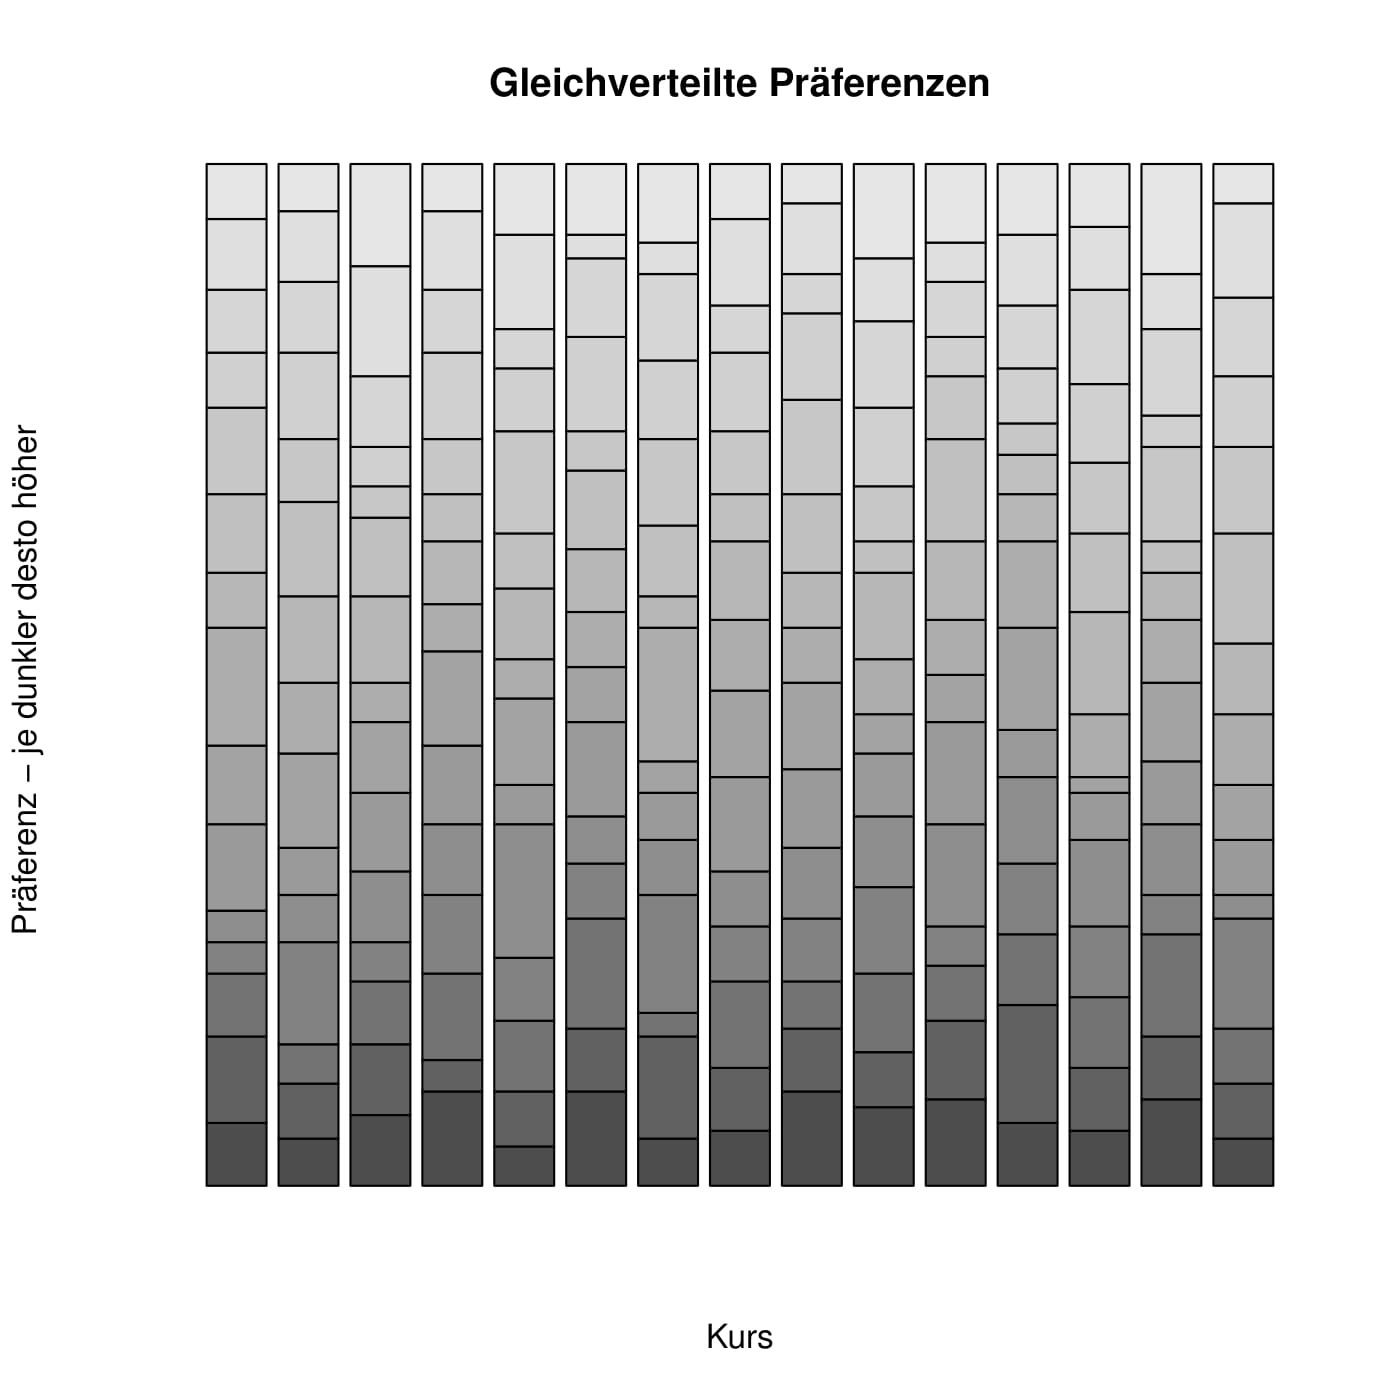
\includegraphics[width=0.7\textwidth]{./testing/images/EqualDistPreferencesDist.jpg}
				\caption{Gleichverteilte Präferenzen mit 130 Studenten auf 15 Kursen mit maximal 10 Teilnehmern pro Kurs. Die Dunkelheit stellt die Höhe der Präferenz dar}
				\label{fig:test_equal_distribution}
			\end{figure}
			Die gleichverteilte Präferenzenmatrix ist in Abbildung \ref{fig:test_equal_distribution} zu sehen.
			
			\begin{figure}
				\centering
				\begin{subfigure}{0.49\textwidth}
					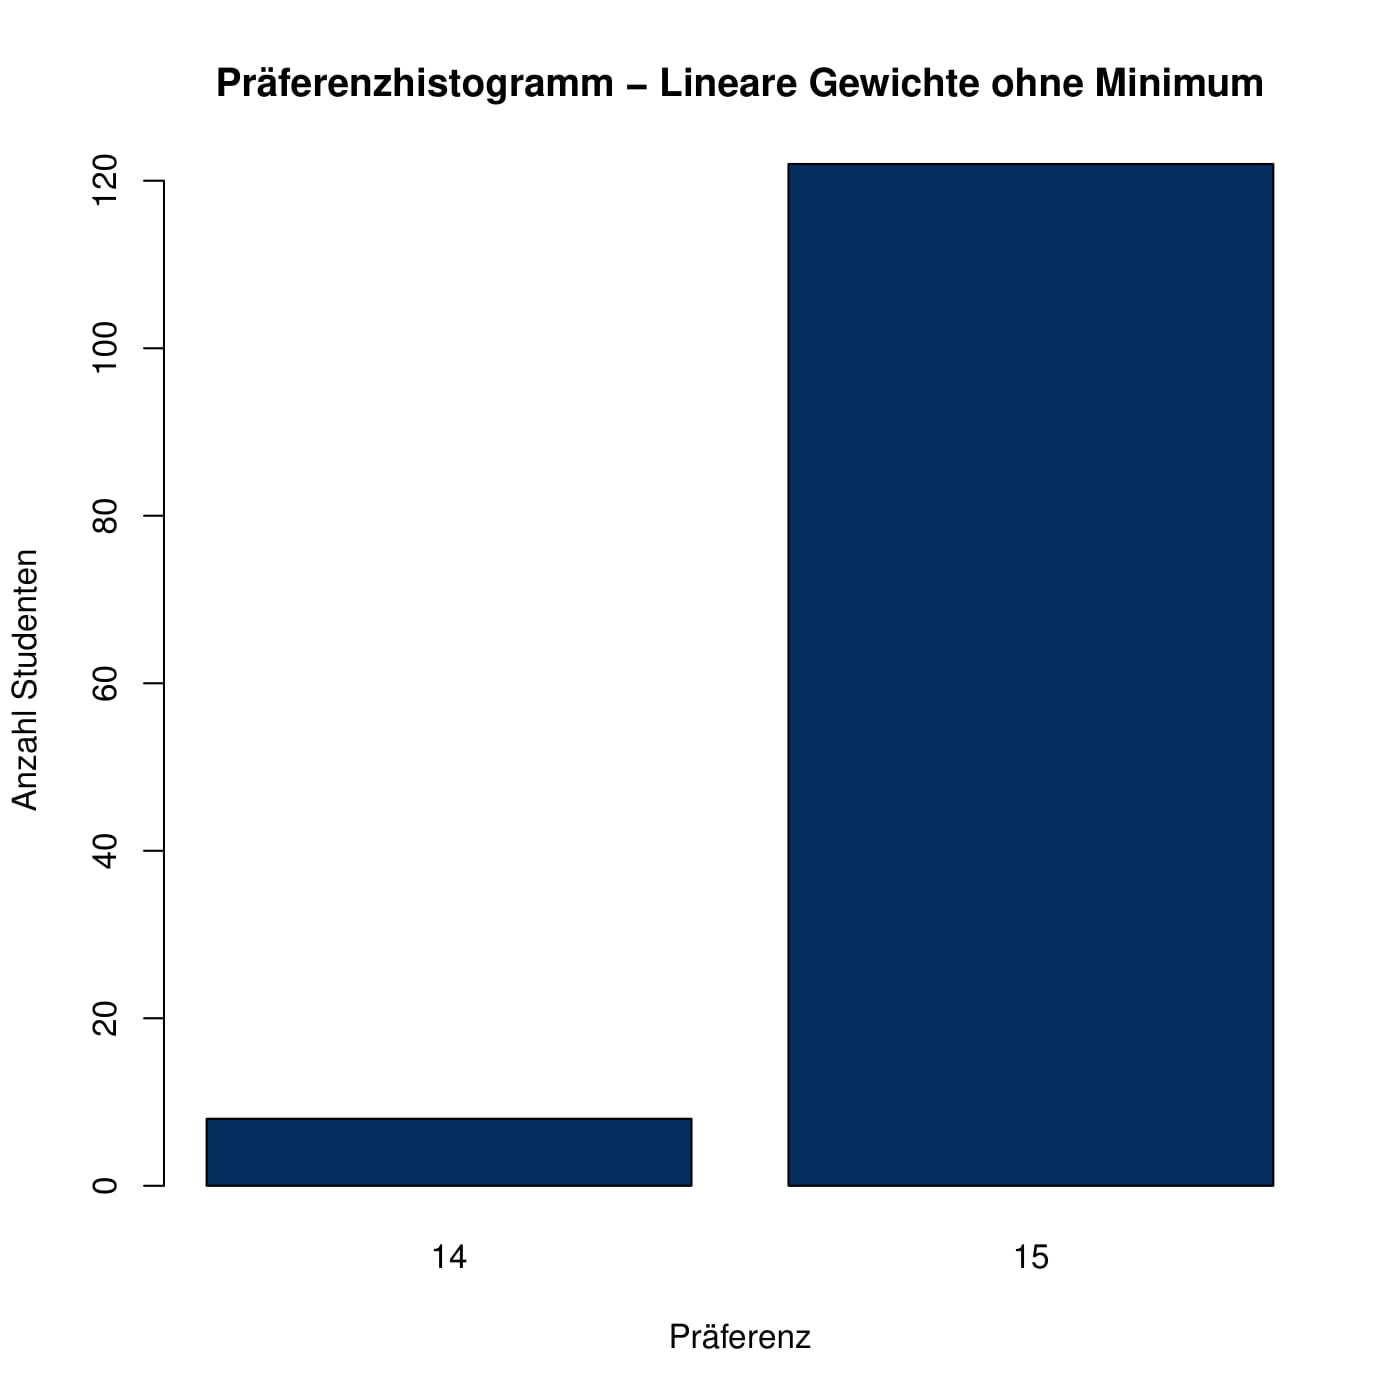
\includegraphics[width=1.0\textwidth]{./testing/images/EqualDistPreferencesHistLin.jpg}
				\end{subfigure}
				\begin{subfigure}{0.49\textwidth}
					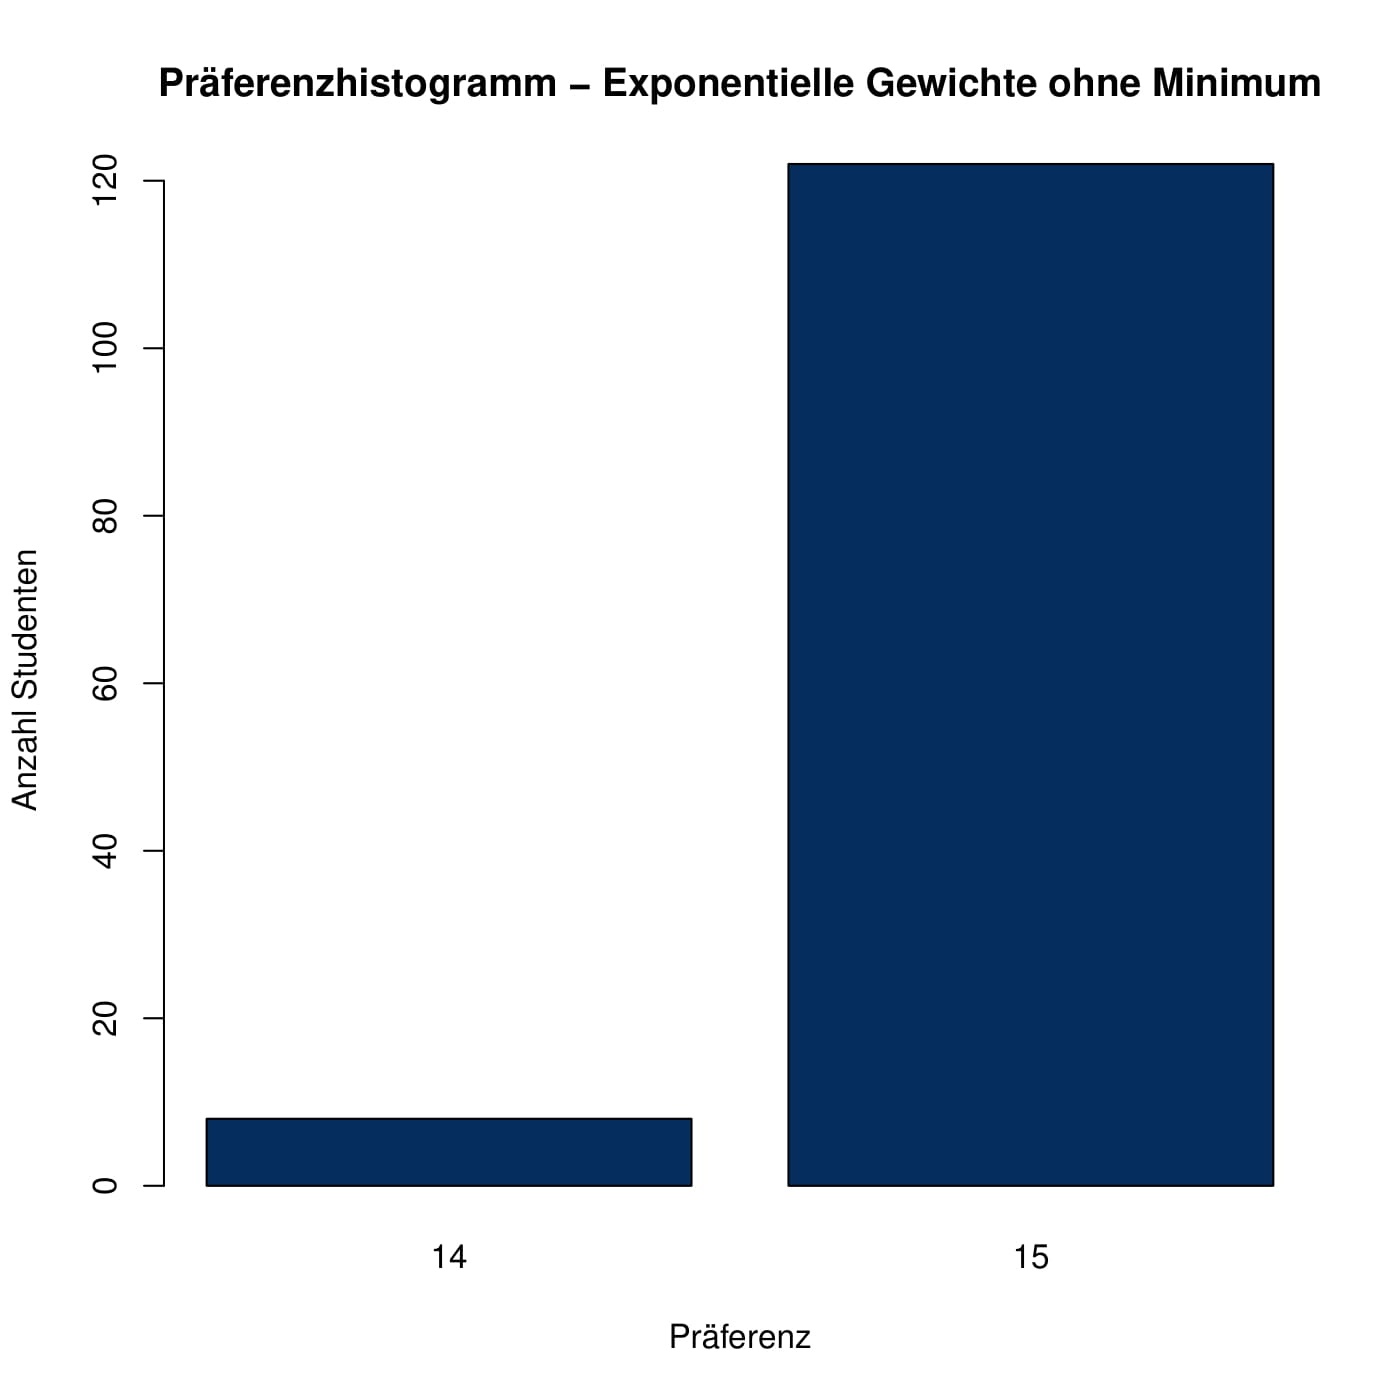
\includegraphics[width=1.0\textwidth]{./testing/images/EqualDistPreferencesHistExpo.jpg}
				\end{subfigure}
				\caption{Gegenüberstellung der Präferenzenhistogramm für lineare und exponentielle Gewichtung}
				\label{fig:test_equal_distribution_histogram}
			\end{figure}
			
			Die Verteilung ist in dem Präferenzenhistogramm in Abbildung \ref{fig:test_equal_distribution_histogram} dargestellt.\newline
			
			Wie man sieht, bekommen die meisten Studenten ihre Erstwahl, das heißt den Kurs mit Präferenz 15.
			Nur sehr wenige Studenten bekommen ihre Zweitwahl, das heißt den Kurs mit Präferenz 14.\newline
			
			Der Grund hierfür ist, dass die Präferenzen auf die Kurse gleichverteilt werden.
			Das heißt, die Wahrscheinlichkeit, dass ein beliebiger Student einen beliebigen Kurs mit beliebiger Präferenz wählt, ist immer gleich.
			Nichtsdestotrotz ist eine gewisse Varianz in der Ziehung der Präferenzen zu beobachten.
			Daher hat jeder Kurs unterschiedlich viele Studenten pro Präferenz.
			Daher kann man davon ausgehen, dass es wenige Studenten geben muss, die nur ihre Zweitwahl kriegen können.\newline
		
		\subsection{Normalverteilung}
		\label{sec:testing:normaldistribution}
		
			\begin{figure}
				\centering
				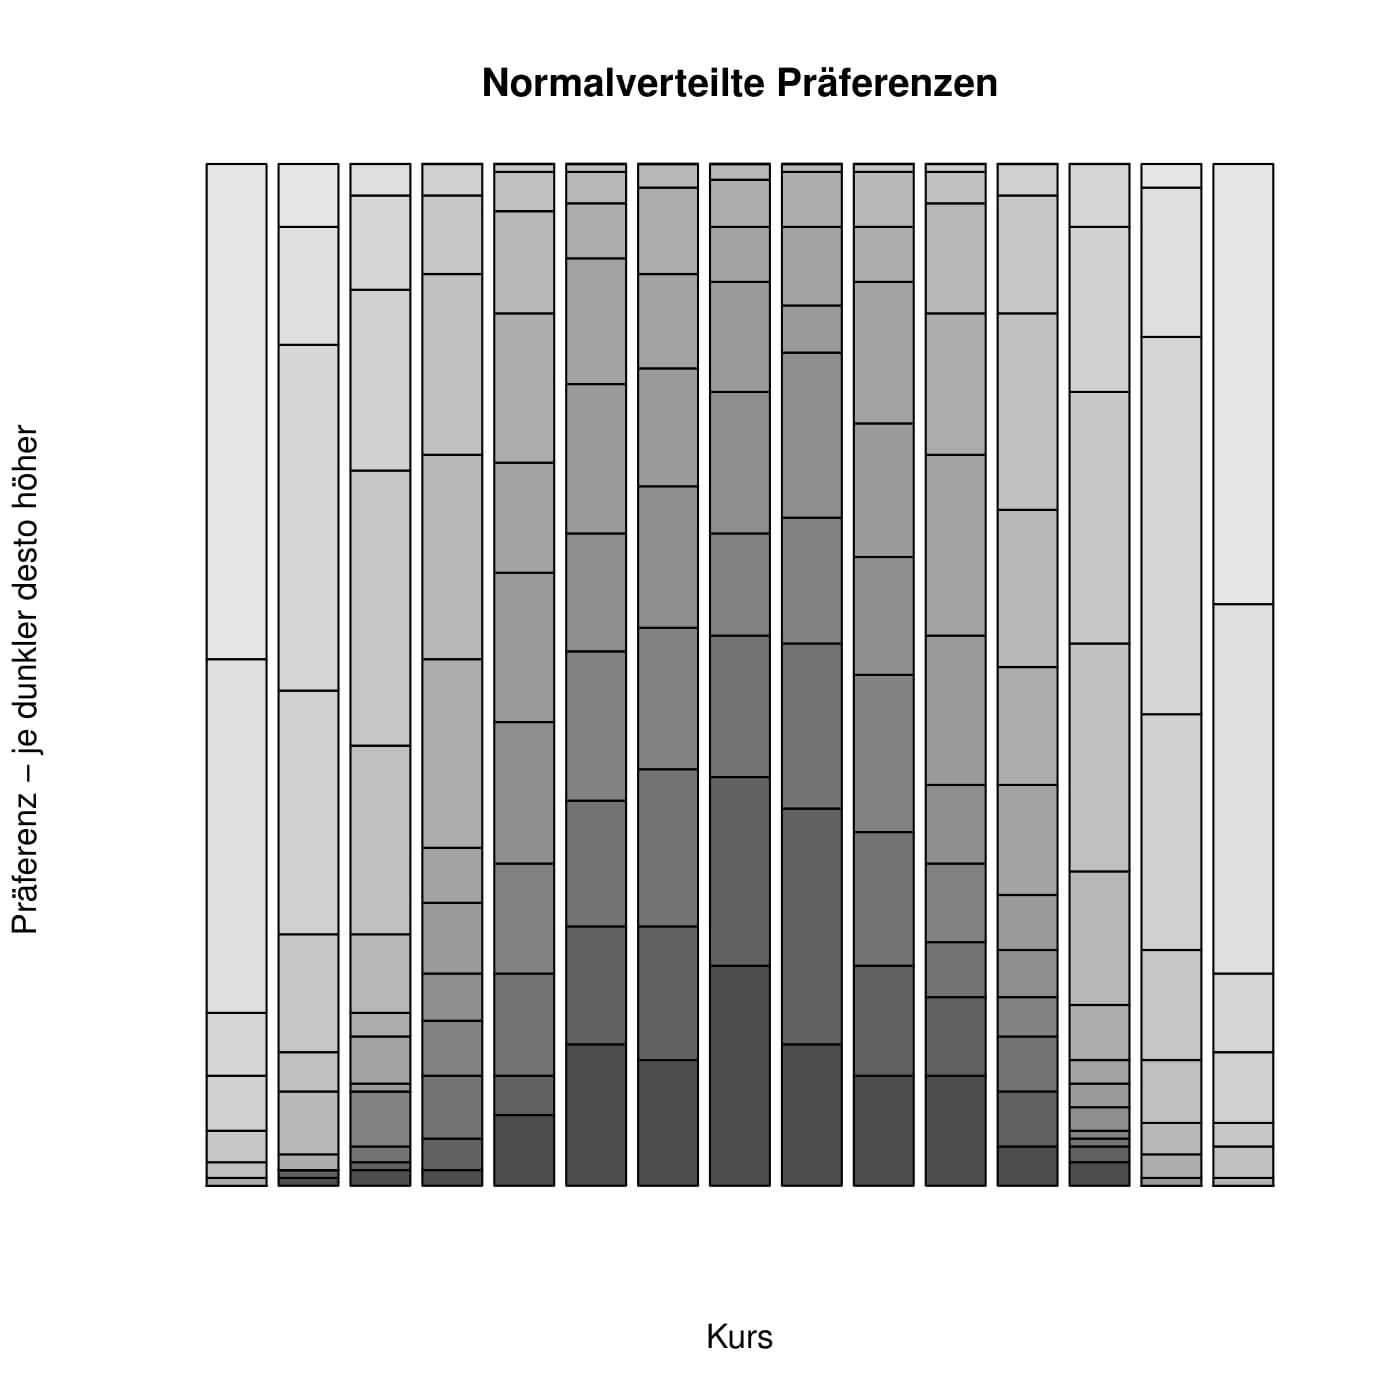
\includegraphics[width=0.7\textwidth]{./testing/images/NormalDistPreferencesDist.jpg}
				\caption{Normalverteilte Präferenzen mit 130 Studenten auf 15 Kursen mit maximal 10 Teilnehmern pro Kurs. Die Dunkelheit stellt die Höhe der Präferenz dar}
				\label{fig:test_norm_distribution}
			\end{figure}
			Die normalverteilte Präferenzenmatrix ist in Abbildung \ref{fig:test_norm_distribution} zu sehen.
			
			\begin{figure}
				\centering
				\begin{subfigure}{0.3\textwidth}
					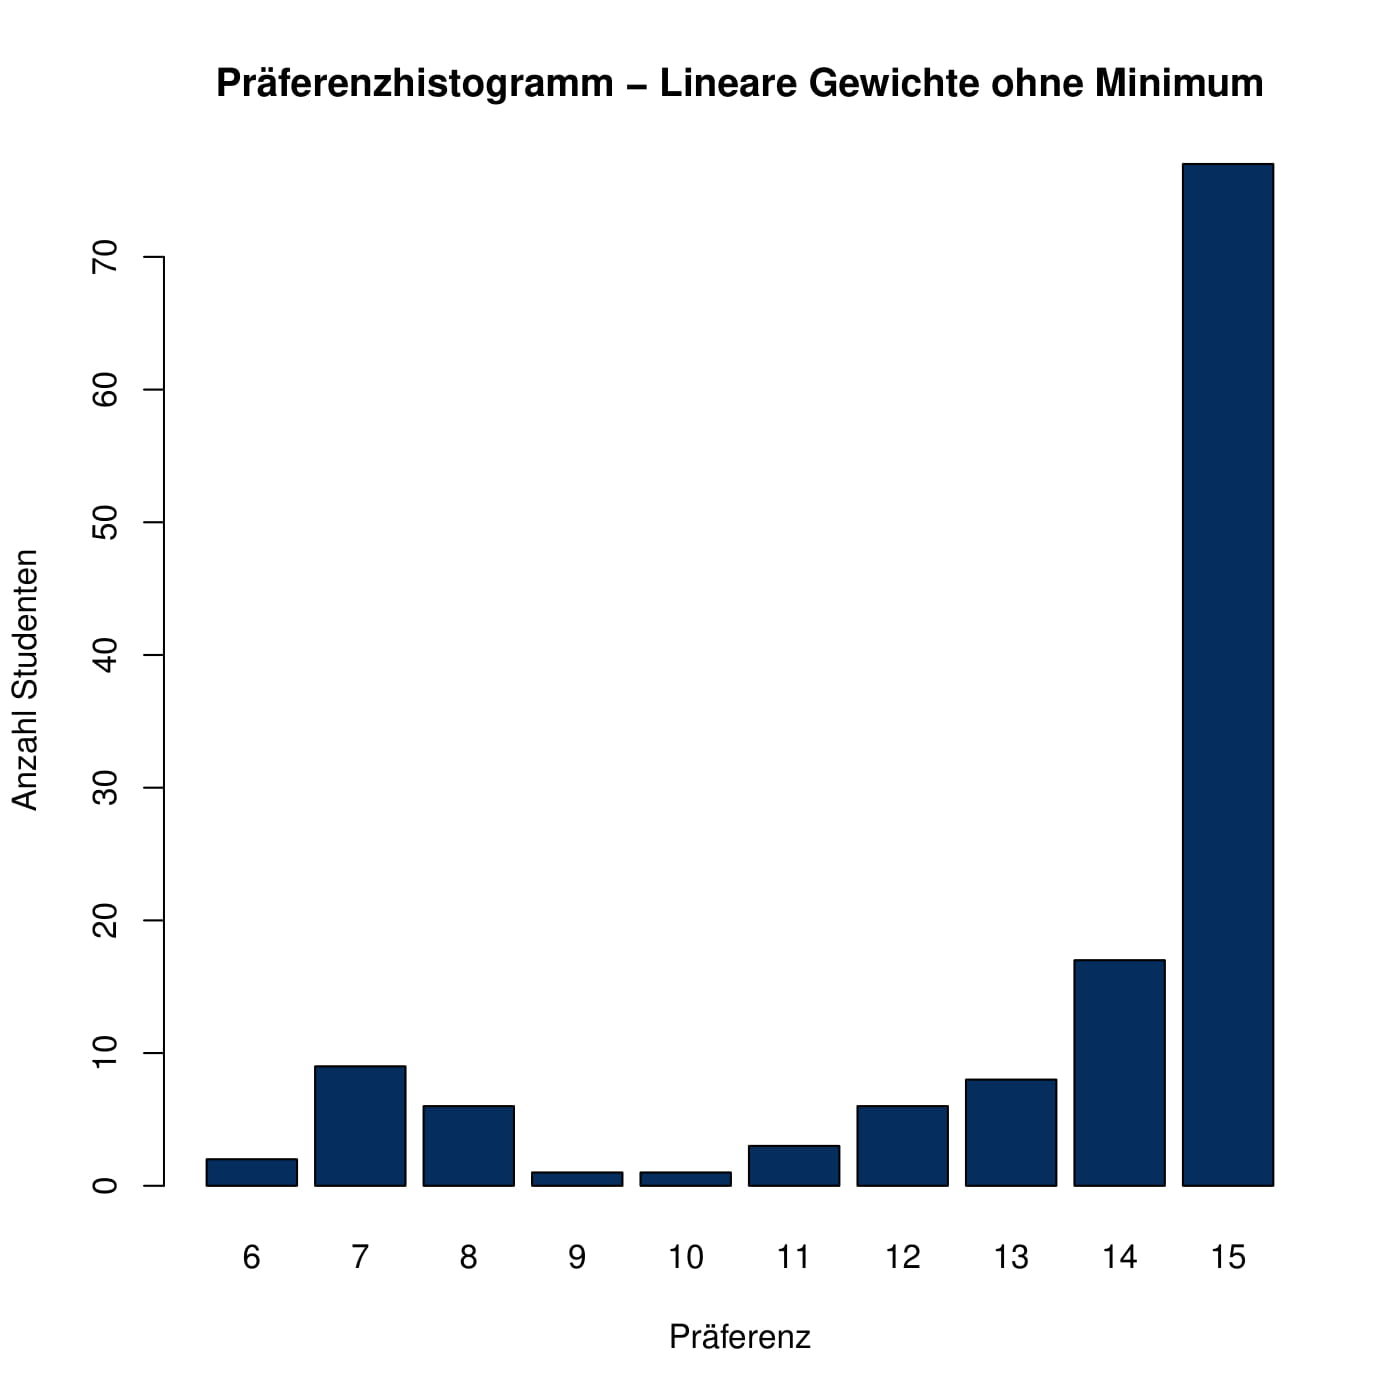
\includegraphics[width=1.0\textwidth]{./testing/images/NormalDistPreferencesHistLin.jpg}
				\end{subfigure}
				\begin{subfigure}{0.30\textwidth}
					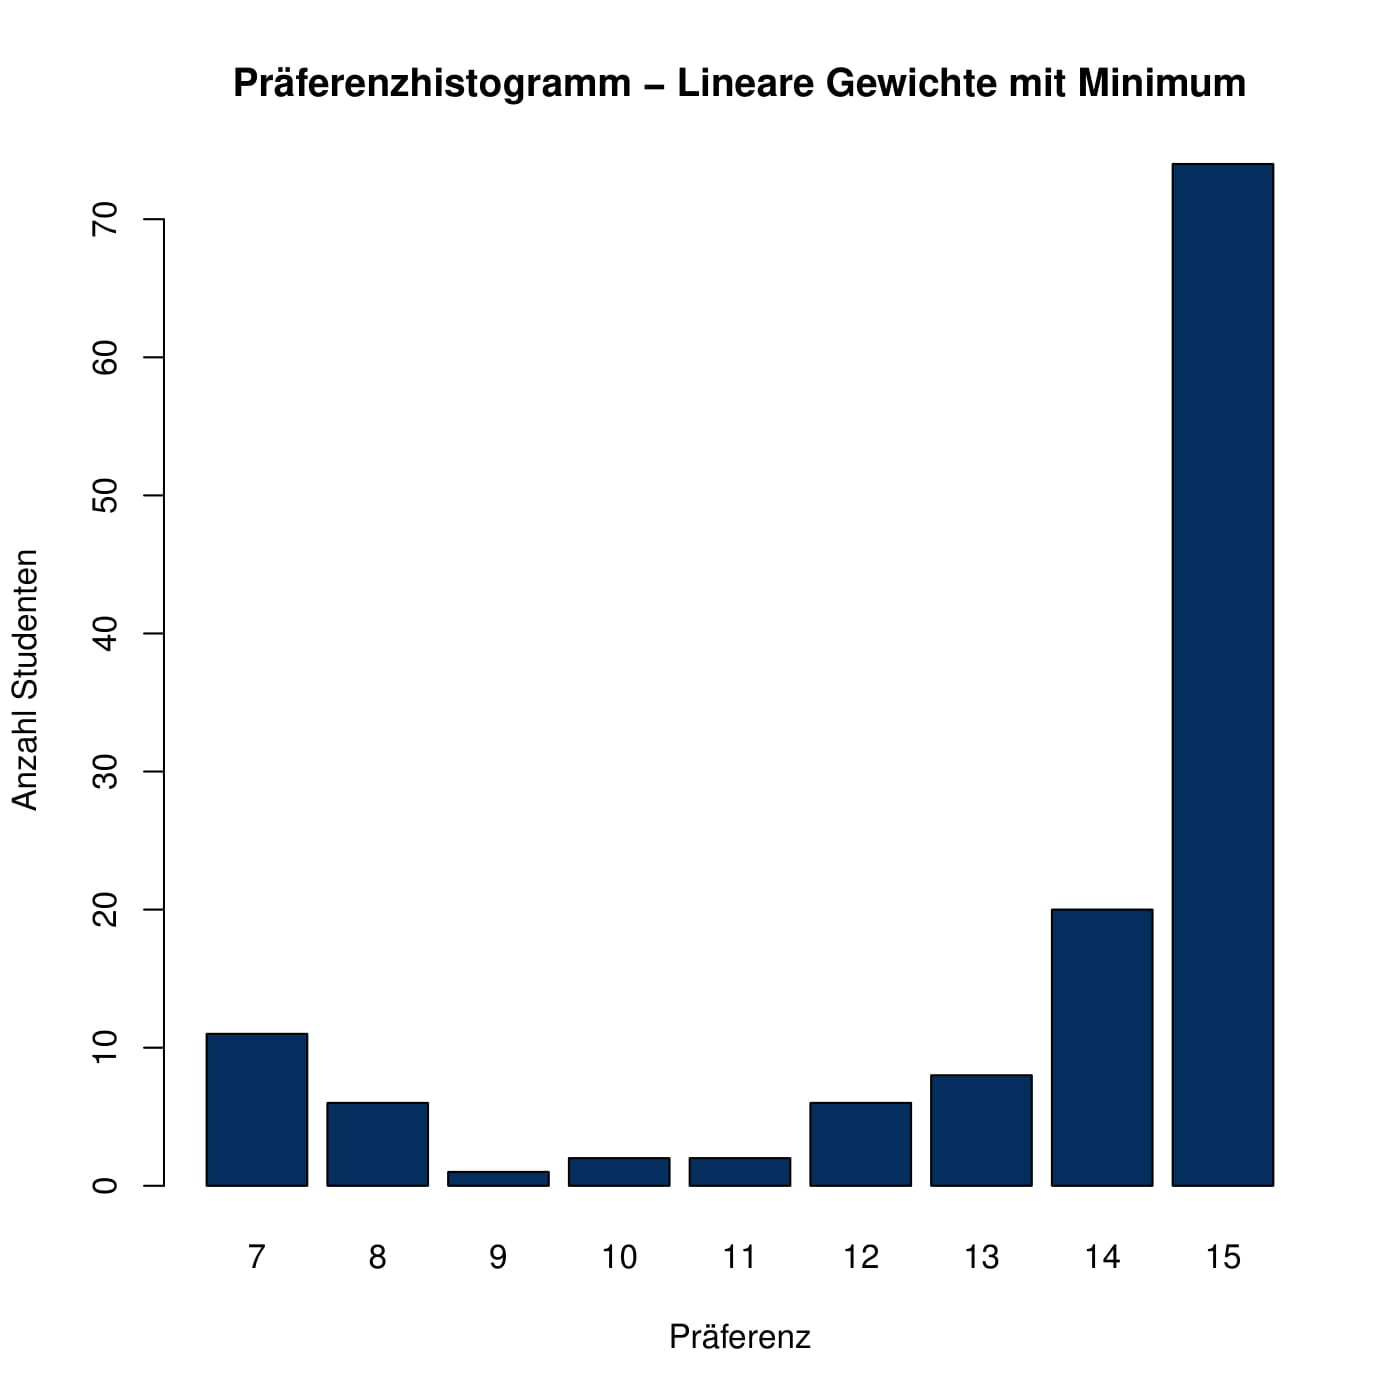
\includegraphics[width=1.0\textwidth]{./testing/images/NormalDistPreferencesHistLinMin.jpg}
				\end{subfigure}
			\begin{subfigure}{0.3\textwidth}
				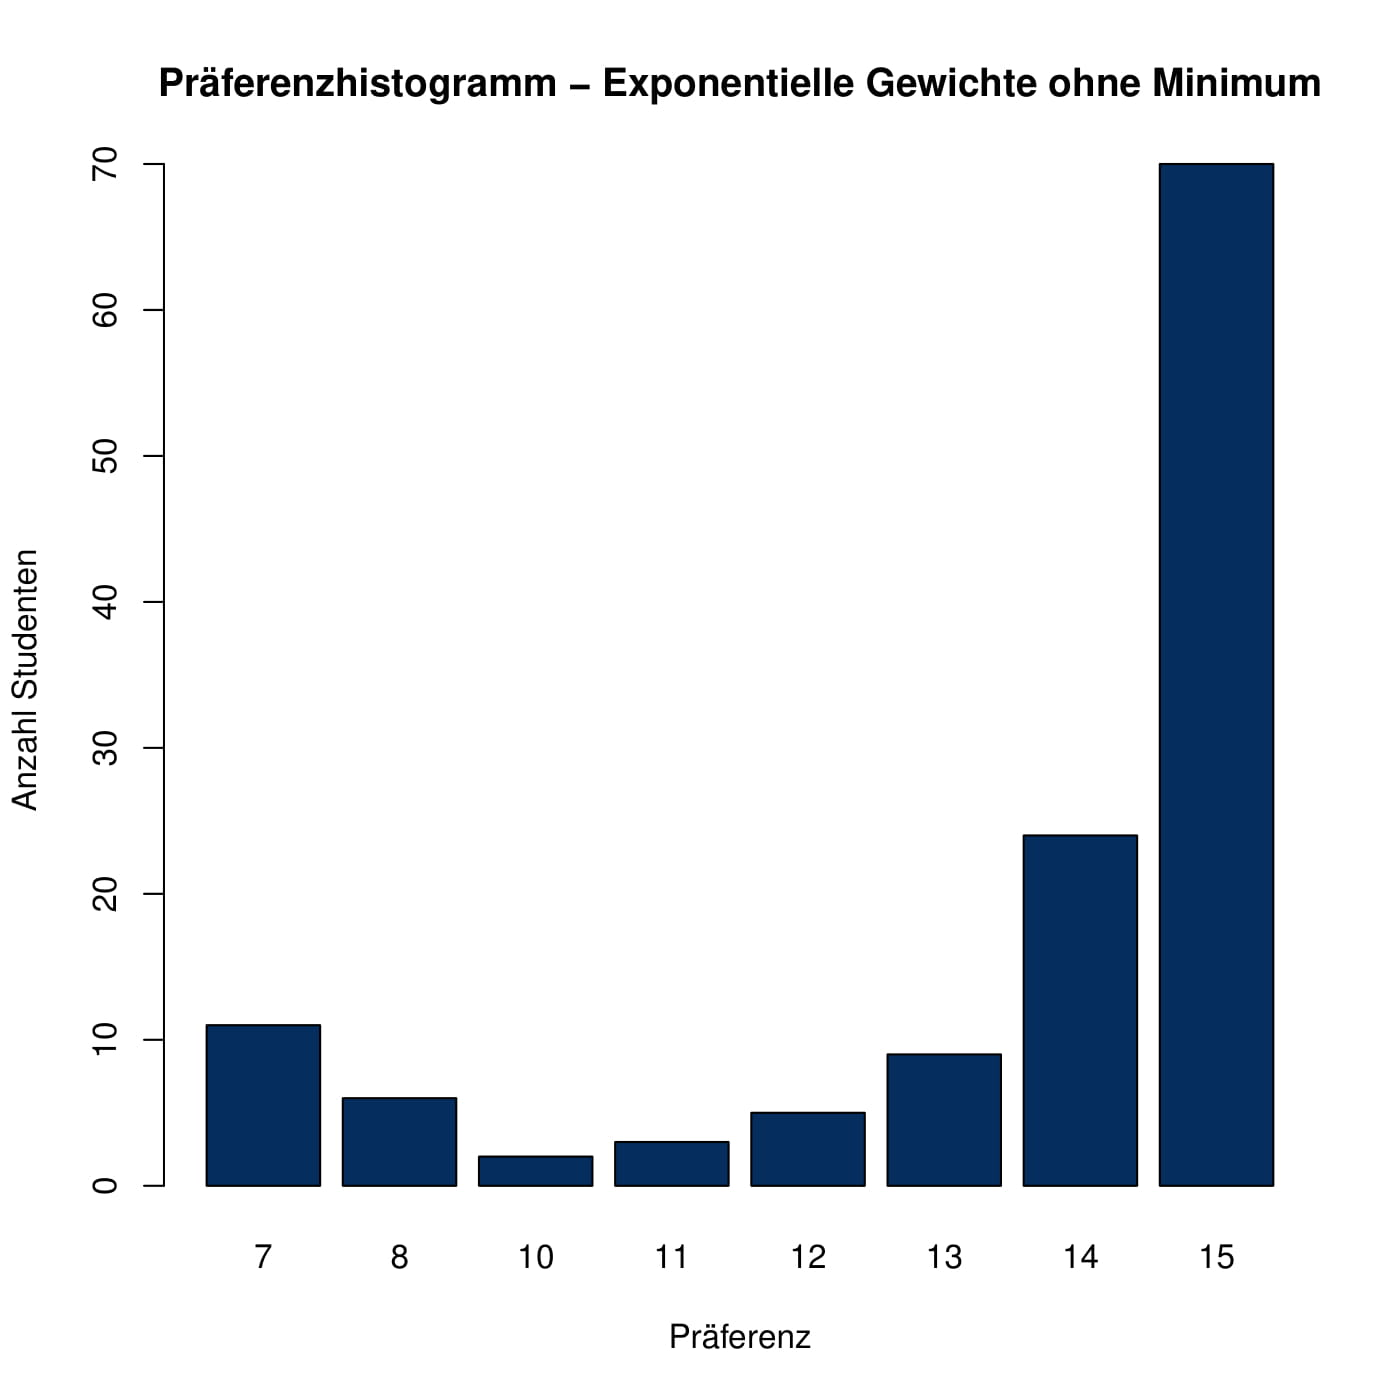
\includegraphics[width=1.0\textwidth]{./testing/images/NormalDistPreferencesHistExpo.jpg}
			\end{subfigure}
				\caption{Gegenüberstellung der Präferenzenhistogramm für lineare Gewichtung, lineare Gewichtung mit Minimum und exponentielle Gewichtung}
				\label{fig:test_norm_distribution_histogram}
			\end{figure}
		
			Die Verteilung ist in dem Präferenzenhistogramm in Abbildung \ref{fig:test_equal_distribution_histogram} dargestellt.\newline
			
			Wie man sieht, bekommen in jeder der Verteilungen mehr als die Hälfte der Studenten ihre Erstwahl.
			Um die 20 Studenten bekommen allerdings nur den Kurs mit einer Präferenz kleiner 11.\newline
			
			Gut zu sehen ist, dass die Variante ''Lineare Gewichte ohne Minimum'' sich von ''Lineare Gewichte mit Minimum'' unterscheidet.
			Die erste Variante hat die minimale Präferenz 6, doch durch das Erzwingen eines festen Minimums verbessert sich diese auf 7.
			Nach den Anforderungen ist dies so wünschenswert.
			Zuletzt ist in der Variante ''Exponentielle Gewichte ohne Minimum'' zu sehen, dass weniger Studenten ihre Erstwahl erhalten, dafür aber mehr Studenten die Präferenz 10 oder höher bekommen.\newline
			
		\subsection{Realdaten}
		
			Letztlich stellte uns der Lehrstuhl, der das Empiriepraktikum leitet, die Daten aus dem Wintersemester 2017/2018 zur Verfügung, um den neuen Algorithmus mit dem alten zu vergleichen.\newline
			
			\begin{figure}
				\centering
				\begin{tabular}{l|l|l}
					& Alter Algorithmus & Neuer Algorithmus \\
					\hline
					Mittelwert & 14.2 & 14.4 \\
					Varianz & 1,8 & 0,75 \\
					Minimale Präferenz & 7 & 12 \\
				\end{tabular}
				\caption{Vergleich des alten Algorithmus mit dem neuen Algorithmus}
				\label{tab:old_versus_new_algorithm}
			\end{figure}
		
			Wie in Abbildung \ref{tab:old_versus_new_algorithm} zu sehen ist, verbessert sich der Mittelwert, die Varianz und minimale Präferenz im Gegensatz zur vorigen Variante.\newline
			
			Dadurch zeigt sich, dass der neue Algorithmus zu einem besseren Ergebnis führt.
			In Folge dessen ist der neue Verteilungsalgorithmus besser als der alte Algorithmus und erfüllt somit das Akzeptanzkriterium.
			
		\subsection{Ergebnisansicht}
			
			Wie in dem Abschnitt \ref{sec:testing:normaldistribution} bereits erklärt, führen die unterschiedlichen Varianten des Algorithmus teilweise zu unterschiedlichen Ergebnissen.
			Wie in den Anforderungen beschrieben, soll der Administrator die Wahl haben, welche dieser Verteilungen er nutzen möchte.
			Daher wurden mehrmals Verteilungen generiert und sicher gestellt, dass die verschiedenen Verteilungen auch tatsächlich so eingetragen werden.
			Da dies sehr aufwendig ist, wurde nur verifiziert, dass die minimale Präferenz auch so im Backend steht.
		
	\section{E-Mail Benachrichtigung}
		Zuletzt wurde die E-Mail-Benachrichtigung getestet.
		Dafür wurde der vorkonfigurierte Mailserver genutzt, der alle E-Mails abfängt.
		Dort konnten alle Mails überprüft werden.
		
		
		
		
		
		
		
		
		
		
		
		
		
		
		
		
		
		
		
		
		
		
		
		
		
